

% LaTeX poster using beamerposter class (3-column layout)
\documentclass[final]{beamer}
\geometry{paperwidth=24in,paperheight=36in}
%\usepackage[margin=2cm]{geometry}
\usepackage{tikz}
\usetikzlibrary{mindmap}
\usepackage{ragged2e} % For \justifying

\usepackage{anyfontsize}
\renewcommand{\normalsize}{\fontsize{18}{22}\selectfont}
% Poster theme and packages
% \usepackage[size=a0,scale=1.0, border=2cm]{beamerposter}
%\usepackage[width=60.96cm,height=91.44cm,scale=1.0]{beamerposter} %setting dimensions to 24 by 36 inches per requirement
\usepackage[size=custom, width=91.44, height=60.96, scale=0.85]{beamerposter}
% \usepackage[width=24in,height=36in,scale=1.0]{beamerposter}
\usepackage{amsmath, amssymb}

\usepackage{graphicx}
\usepackage{xcolor}
\usepackage{multicol}
\usepackage{tikz}
\usetikzlibrary{positioning} % <-- added for 'of=' syntax in tikz
\usepackage[utf8]{inputenc} % Ensure unicode compatibility
\usepackage{lmodern} % Better font rendering for large fonts
% \usepackage{showframe} % Temporary

% Custom NYU Violet color and styling
\definecolor{nyuviolet}{RGB}{87, 0, 140}
\setbeamercolor{block title}{bg=nyuviolet, fg=white}
\setbeamercolor{block body}{bg=white, fg=black}
\setbeamerfont{block title}{series=\bfseries}
% Define the university color from University website
\definecolor{uniLightViolet1}{HTML}{ab82c5}
\definecolor{uniLightViolet2}{HTML}{eee6f3}

%% FOR colors used in equations:
\definecolor{myred}{RGB}{200,0,0}
\definecolor{myblue}{RGB}{0,0,180}
% define a big fat red todo command
\newcommand{\todo}[1]{\textcolor{myred}{\textbf{TODO:} #1}}

% Title and authors
\title{On the Difficulty of Training Recurrent Neural Networks (ICML 2013)}
\author{Razvan Pascanu, Tomas Mikolov, Yoshua Bengio}
%\institute{ICML 2013}

\setbeamerfont{block title}{size=\large, series=\bfseries}
\setbeamerfont{block body}{size=\normalsize}

% Document
\begin{document}

\begin{frame}[t]


\begin{center}
  \noindent
  \colorbox{nyuviolet}{\parbox{\textwidth}{\centering
    % Overlay logo on the left
    \begin{tikzpicture}[remember picture, overlay]
      \node[anchor=north west, inner sep=0pt] at ([xshift=1.5cm, yshift=-2.5cm]current page.north west) {
        
\includegraphics[width=0.2\textwidth, valign=c]{figures/cds_logo.png}
      };
    \end{tikzpicture}
    % Centered text
    \color{white}
    \Huge\bfseries On the Difficulty of Training RNNs (ICML, 2013)\\[0.5em]
    \Large R. Pascanu, T. Mikolov, Y. Bengio\\[0.7em]
    \large \textit{Poster presented by: Hanna M. Dettki, Anagha Radhakrishna Palandye, Juechen Zhong, Harshit Bhargava}
  }}
\end{center}




  \begin{columns}[t,totalwidth=\textwidth]

    %%%%%%%%%%%%%%%%%%%%%%%%%%%%%%%%%%%% Column 1 %%%%%%%%%%%%%%%%%%%%%%%%%%%%%%%%%%%%%%%%%%%%%%%%%%%%%%%%
    \hspace{0.05cm}
    \begin{column}{0.3\textwidth}
      \begin{block}{1. Introduction \& Background}

        \textbf{1.1 Context \& Motivation}
            \begin{itemize}
            \item \textbf{Importance of sequence modeling}
            \begin{itemize}
                \item e.g., language, time-series in finance
            \end{itemize}

            \item Identifying gradient problems [1]%(Bengio et al., 1994)
            \begin{itemize}
                \item \textbf{Vanishing gradient problem (VGP)}: impossible to learn long-term dependencies
                \item \textbf{Exploding gradient problem (EGP)}: numerical instabilities $\rightarrow$ unstable training
            \end{itemize}

            % \item $\rightarrow$ a) Why stable gradient flow is critical for learning temporal dependencies; b) and solutions (both paper's contribution)
            \item $\rightarrow$ \textbf{a.} 
            %Stable gradient propagation as a prerequisite for learning long-range dependencies in RNNs
            Why learning long-term dependencies requires stable gradients
\textbf{b.} Gradient norm clipping \& temporal sensitivity regularization as  solutions for VGP \& EGP (both \textbf{a} \& \textbf{b} are paper's contributions)
            \end{itemize}

        % \vspace{1em}

        \textbf{1.2 Schematic \& formal def. of a Recurrent Neural Network (RNN)}


        \begin{center}
            \begin{tikzpicture}[node distance=2.5cm, thick, >=latex, every node/.style={scale=1.5}, xshift=-1cm]
       % Nodes
       \node[draw, minimum height=1.5cm, minimum width=0.8cm] (input) {$u_t$};
       \node[draw, right=of input, minimum height=1.5cm, minimum width=0.8cm] (rnn) {$x_t$};
       \node[right=of rnn] (error) {$\mathcal{E}_t$};
       
       % Arrows
       \draw[->, line width=1.5pt] (input) -- (rnn);
       \draw[->, line width=1.5pt] (rnn) -- (error);
       
       % Recurrent loop (from right to left, meeting top corners)
       \draw[->, orange, line width=2pt]
           ([xshift=3pt,yshift=3pt]rnn.north east)
           to[out=45,in=135,looseness=1.2]
           ([xshift=-3pt,yshift=3pt]rnn.north west);
       % Label
       % \node[below=0.5cm of input] {\tiny{Fig. 1: \textcolor{orange}{\textbf{The recurrent connections}} in the hidden layer allow information to persist from one input to another.}}
       ;
       \end{tikzpicture}
       \end{center}
       \vspace{-.6em}
{{Fig. 1: \textcolor{orange}{\textbf{The recurrent connections}} in the hidden layer allow information to persist from one input to another.}}
   % \vspace{.5em}
   \begin{align*}
     x_t &= F(x_{t-1}, u_t, \theta) && \text{(1) General} \\
     x_t &= \textcolor{orange}{W_{\text{rec}}} \, \sigma(x_{t-1}) + W_{in} u_t + \mathbf{b} && \text{(2) used in the paper}
   \end{align*}

        \vspace{0.5em}
        %\small
        where $\bullet$ $u_t$: input, $\bullet$  $x_t$: state, $\bullet$  $t$: time step, $\bullet$  $\mathbf{b}$: bias,  $\bullet$  $\mathcal{E}_t = \mathcal{L}(x_t)$ (error),  $\bullet$  \textcolor{orange}{$W_{rec}$: recurrent weight matrix}

        \vspace{0.5em}
        %\textcolor{orange}{\textbf{The recurrent connections}} in the hidden layer allow information to persist from one input to another.

        % \vspace{1em}
        \textbf{1.3 Training RNNs: Backprop Through Time (BPTT) on Unrolled RNN}\\
        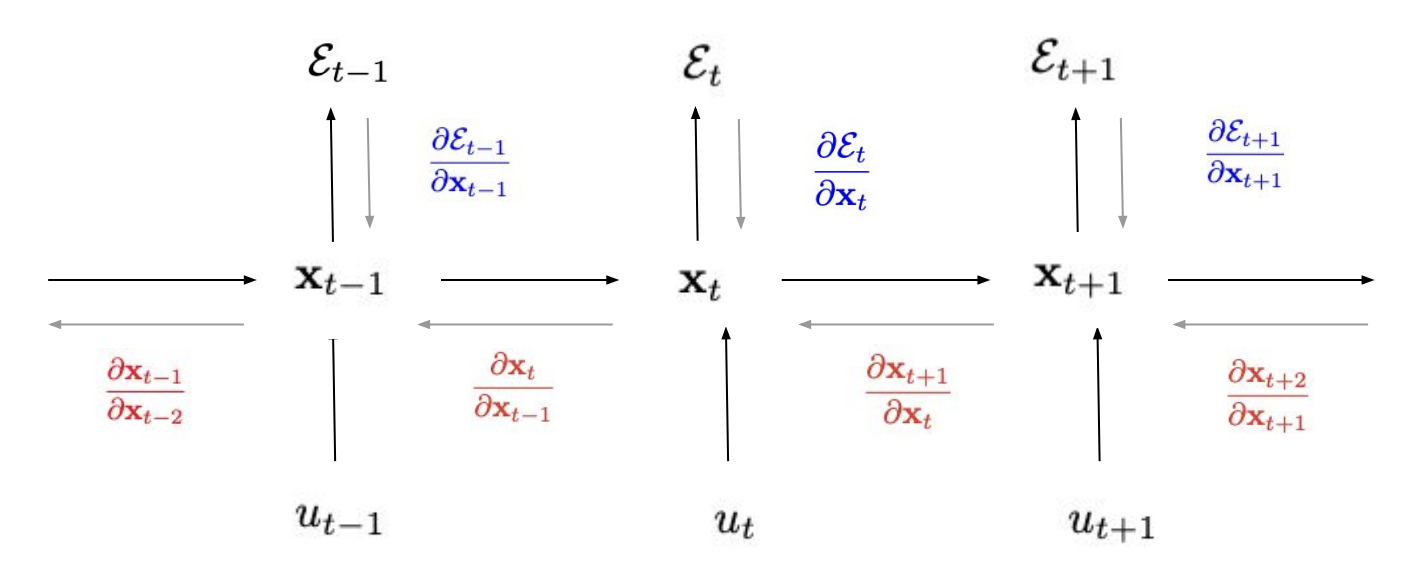
\includegraphics[width=0.95\linewidth]{figures/RNN.png} \\[0.3em]
         Fig. 2: Unrolled RNN: Creating a copy of the model for each time step. \textcolor{myblue}{$\mathcal{E}_t$:}  error obtained at time step $t$ from the output |
          %\Pseudo-code{3em} 
          $\bullet$ \textcolor{myblue}{ \textit{total gradient over time}}
        \quad
        $\bullet$ \textcolor{myred}{ \textit{temporal error contribution}}


        \vspace{-0.6em}
        \begin{align*}
          \textcolor{myblue}{\frac{\partial \mathcal{E}}{\partial \theta}} &=
          \sum_{t=1}^{T} \frac{\partial \mathcal{E}_t}{\partial \theta} \hspace{2em} \text{(3)} \\[0.5em]
          \frac{\partial \mathcal{E}_t}{\partial \theta} &=
          \sum_{k=1}^{t} 
          \left( {\frac{\partial \mathcal{E}_t}{\partial x_t}} 
          \textcolor{myred}{\frac{\partial x_t}{\partial x_k}}
          \frac{\partial^+ x_k}{\partial \theta} \right) \hspace{2em} \text{(4)} \\[0.5em]
          \textcolor{myred}{\frac{\partial x_t}{\partial x_k}} &=
          \prod_{i=k+1}^{t}
          \textcolor{orange}{W_{\text{rec}}}^\top \cdot \text{diag}\left(\sigma'(x_{i-1})\right) \hspace{2em} \text{(5)}
        \end{align*}
        
        % \vspace{0.5em}
        where $\frac{\partial^+ x_k}{\partial \theta}$ denotes the “immediate” partial derivative (treating $x_{k-1}$ as constant).
        %$\bullet$ \textcolor{myblue}{ \textit{total gradient over time}}
        % \quad
        %$\bullet$ \textcolor{myred}{ \textit{temporal error contribution}}

      \end{block}

      \begin{block}{2. The Problem}

    \textbf{2.1 Mechanics of Exploding and Vanishing Gradients:}
\justifying{
\begin{itemize}
    \item \justifying These issues occur in RNNs due to repeated multiplication of Jacobian matrices during backpropagation.
    \item \justifying The behavior of gradients depends on the spectral radius $\rho$ of the recurrent weight matrix $W_{\text{rec}}$:
    \begin{itemize}
        \item If $\rho < 1$, gradients \textbf{vanish}.
        \item If $\rho > 1$, gradients \textbf{explode}.
    \end{itemize}
    \item \justifying For non-linear activations with bounded derivatives (e.g., $\gamma = 1$ for \texttt{tanh}), gradients \textbf{vanish} when the largest singular value $\lambda_1 < \gamma^{-1}$.
\end{itemize}
}
    \end{block}
    \end{column}

   %%%%%%%%%%%%%%%%%%%%%%%%%%%%%%%%%%%% Column 2 %%%%%%%%%%%%%%%%%%%%%%%%%%%%%%%%%%%%%%%%%%%%%%%%%%%%%%%%
\begin{column}{0.3\textwidth}
    \begin{block}{2. The Problem (cont.)}

    % \vspace{0.5em}
\textbf{2.2 Dynamical Systems View:} \\
\justifying{
    \begin{itemize}
        \item \justifying An RNN's hidden state evolves like a dynamical system converging to attractors.
        \item \justifying As parameters change, the system may cross bifurcation points, causing drastic changes in state evolution.
        \item \justifying Crossing basin boundaries can result in gradient explosions.
        \item \justifying Inputs can shift the system into different attractor basins, intensifying this instability.
    \end{itemize}
    
}

    \begin{center}
\begin{minipage}[t]{0.45\linewidth}
    \centering
    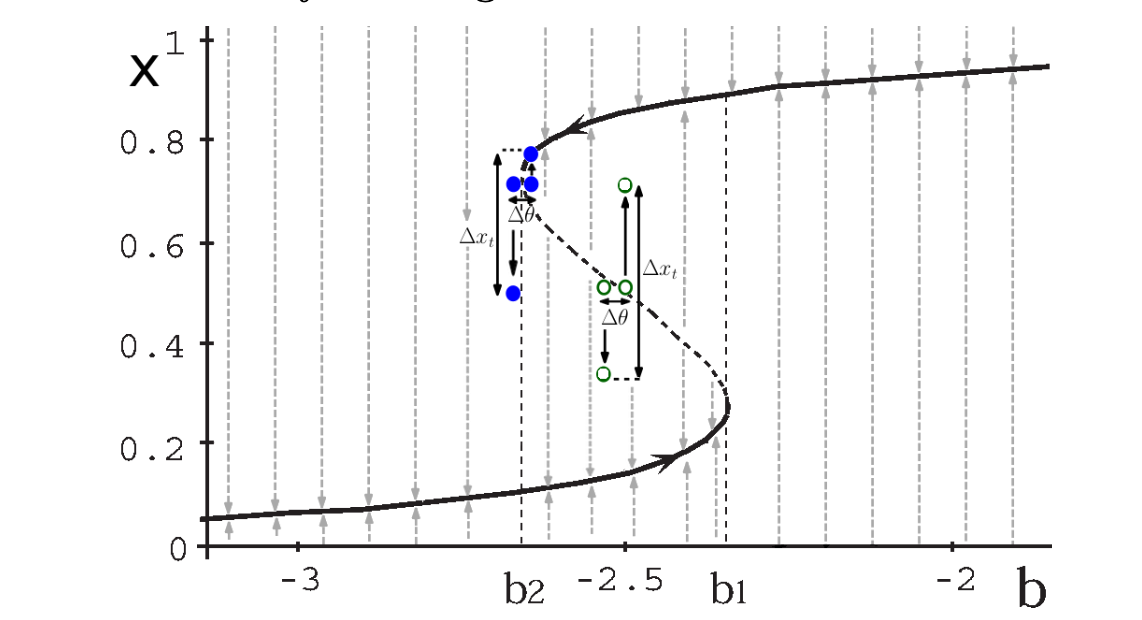
\includegraphics[width=\linewidth]{figures/bifurcation.png} \\
    \small Fig.3:Bifurcation for attractor transitions
\end{minipage}
\hfill
\begin{minipage}[t]{0.45\linewidth}
    \centering
    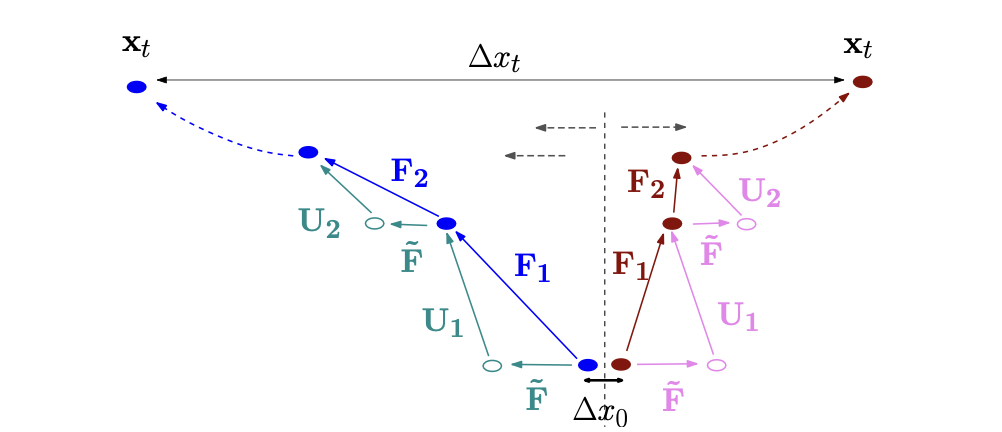
\includegraphics[width=\linewidth]{figures/function_and_input.png} \\
    \small Fig.4:Grad explosion due to basin crossing
\end{minipage}
\end{center}


    \vspace{0.5em}
        \textbf{2.3 Geometric Interpretation:}

        % \vspace{0.1em} % optional: adds spacing below the title

        \begin{minipage}[t]{0.54\textwidth}
        \begin{itemize}
                \item \justifying Consider $x_t = w\sigma(x_{t-1}) + b$ with $x_0 = 0.5$.
                \item \justifying In the linear case ($b = 0$), gradients are $\frac{\partial x_t}{\partial w} = t w^{t-1} x_0$, showing exponential growth.
                \item \justifying Exploding gradients align with steep directions in the error surface.
                \item \justifying These steep directions form sharp walls that SGD struggles to traverse, disrupting convergence.
        \end{itemize}
        
        \end{minipage}%
        \hfill
        \begin{minipage}[t]{0.45\textwidth}
          \centering
          \vspace{-1em} % pull image up to align with first bullet
          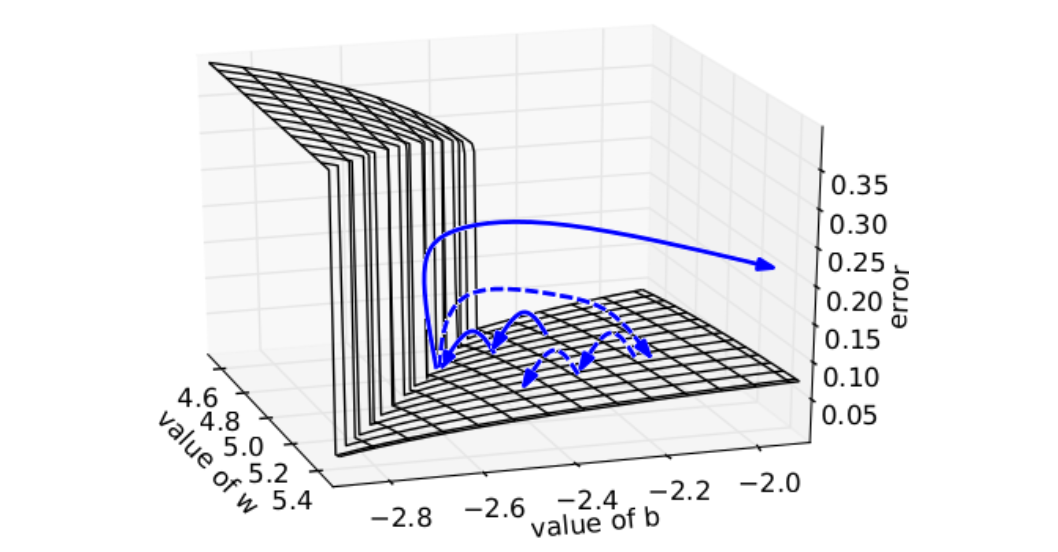
\includegraphics[width=\linewidth]{figures/geometric.png}
          
        \vspace{0.3em} % spacing between image and caption
        {\small Fig.5:Steep error surface caused by exploding gradients}
    \end{minipage}
    \end{block}
    
        
%     \textbf{2.3 Geometric Interpretation:} \\
% \justifying{
% \begin{itemize}
%     \item \justifying Consider $x_t = w\sigma(x_{t-1}) + b$ with $x_0 = 0.5$.
%     \item \justifying In the linear case ($b = 0$), gradients are $\frac{\partial x_t}{\partial w} = t w^{t-1} x_0$, showing exponential growth.
%     \item \justifying Exploding gradients align with steep directions in the error surface.
%     \item \justifying These steep directions form sharp walls that SGD struggles to traverse, disrupting convergence.
% \end{itemize}
% }
%     \begin{center}
% \begin{minipage}[t]{0.48\linewidth}
%     \centering
%     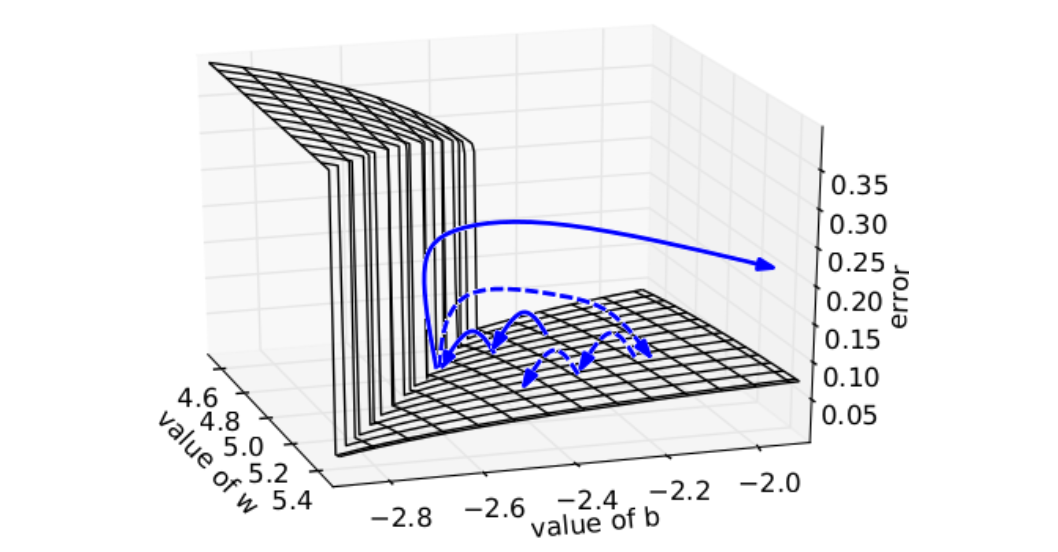
\includegraphics[width=\linewidth]{figures/geometric.png} \\
%     \small Fig 5.Steep error surface by exploding gradients
% \end{minipage}
% \end{center}

%     \end{block}
    \begin{block}{3. Solutions }

        \textbf{3.1 Gradient Clipping}
            
        \begin{minipage}{0.54\textwidth}
        \begin{itemize}
          \item \justifying Pseudo-code: $\hat{g} \leftarrow \nabla E;\ \text{if } \|\hat{g}\|_2 \geq \tau \text{ then } \hat{g} \leftarrow \tau \cdot \frac{\hat{g}}{\|\hat{g}\|_2}$
          \item \justifying Gradient clipping introduces a hyperparameter: the threshold. A common heuristic sets this value based on the average gradient norm over early training steps.
          \item \justifying Compared to clipping individual gradient components by value, norm-based clipping preserves the direction of the gradient vector and is generally more robust in high-dimensional settings.
        \end{itemize}
        \end{minipage}
        \hfill
        \begin{minipage}{0.45\textwidth}
        \centering
        \vspace{1em} % pulls the image up
        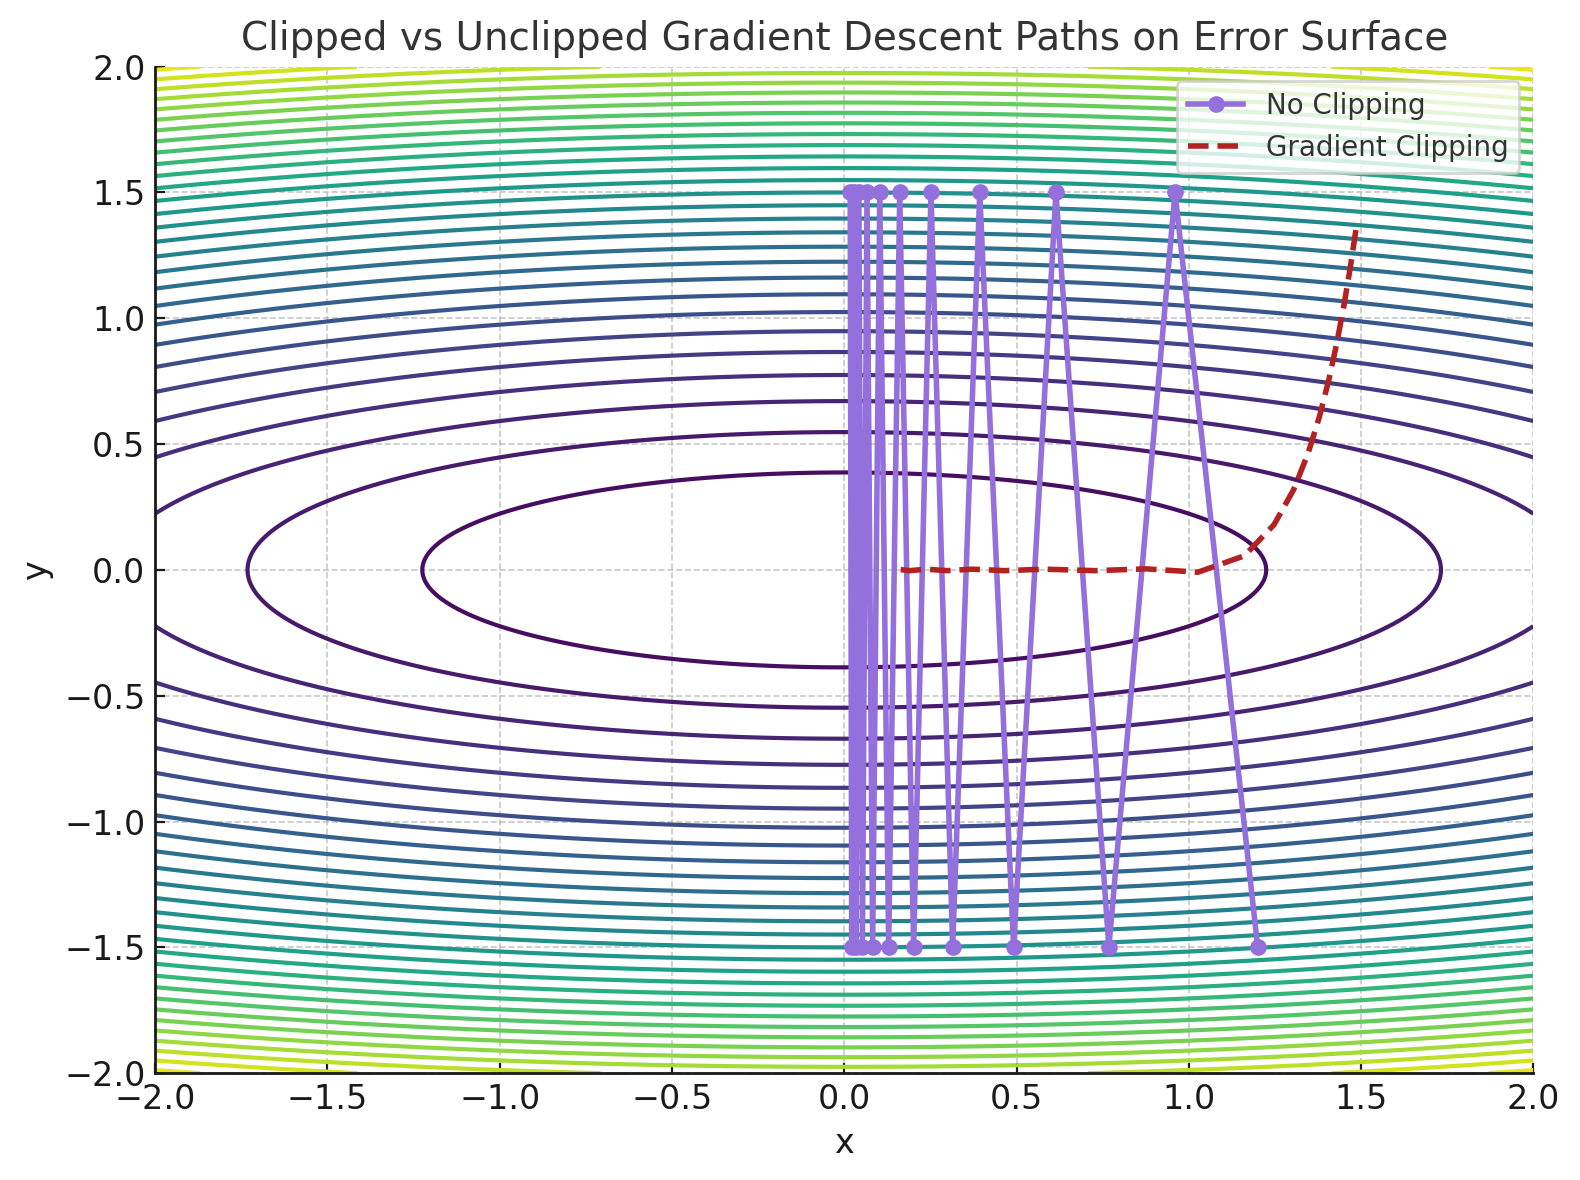
\includegraphics[width=\linewidth]{figures/gradient_clipping.png}
        \small Fig.6:Clipped vs Unclipped Gradient Descent Path on Error Surface
        \end{minipage}
        
    \textbf{3.2 Vanishing Gradient Regularization}
      \begin{itemize}
        \item \justifying Regularizer: 
            \begin{align*}
            \Omega &= \sum_k \Omega_k 
            = \sum_k \left(  
            \frac{ \left\| \frac{\partial \mathcal{E}}{\partial x_{k+1}} 
            \cdot \frac{\partial x_{k+1}}{\partial x_k} \right\| }
            { \left\| \frac{\partial \mathcal{E}}{\partial x_{k+1}} \right\| } - 1 
            \right)^2 \hspace{2em} \text{(6)} \\[1em]
            %
            \frac{\partial^+ \Omega}{\partial W_{\text{rec}}} &= \sum_k 
            \frac{\partial^+}{\partial W_{\text{rec}}} \left[
            \left( 
            \frac{ \left\| \frac{\partial \mathcal{E}}{\partial x_{k+1}} 
            \cdot W_{\text{rec}}^\top 
            \cdot \operatorname{diag}\left( \sigma'(x_k) \right) \right\|^2 }
            { \left\| \frac{\partial \mathcal{E}}{\partial x_{k+1}} \right\|^2 } - 1 
            \right)^2
            \right] \hspace{2em} \text{(7)}
            \end{align*}

            % \Omega = \sum_k \Omega_k = \sum_k \left(  \frac{ \left\| \frac{\partial E}{\partial x_{k+1}} \cdot \frac{\partial x_{k+1}}{\partial x_k} \right\| }
            % { \left\| \frac{\partial E}{\partial x_{k+1}} \right\| } - 1 
            % \right)^2
            % \]
            % \[
            % \textstyle
            % \frac{\partial^+ \Omega}{\partial W_{\text{rec}}} = \sum_k 
            % \frac{\partial^+}{\partial W_{\text{rec}}} \left(
            % \left( 
            % \frac{ \left\| \frac{\partial E}{\partial x_{k+1}} \cdot W_{\text{rec}}^\top \cdot \operatorname{diag}\left( \sigma'(x_k) \right) \right\|^2 }
            % { \left\| \frac{\partial E}{\partial x_{k+1}} \right\|^2 } - 1 
            % \right)^2
            % \right)
            % \]
        \item \justifying The regularization term only enforces norm preservation of the Jacobian matrix
        $\frac{\partial x_{k+1}}{\partial x_k}$ in the direction of the error signal 
        $\frac{\partial \mathcal{E}}{\partial x_{k+1}}$, not in all directions.
        
        \item \justifying The soft constraint does not guarantee perfect norm preservation, so exploding gradients may still occur, particularly during early training or unstable updates. To mitigate this, we combine the regularizer with gradient clipping for more stable and effective learning.

        \end{itemize}
    \end{block}
\end{column}

    % Column 3
    \begin{column}{0.3\textwidth}
    \begin{block}{4. Experiments \& Results}

    \begin{itemize} 
    \item \justifying \textbf{Datasets Utilized:} Synthetic pathological tasks (temporal order, addition, multiplication, 3-bit temporal order, random permutation, noiseless memorization)[2]. Natural datasets polyphonic music prediction [3](Piano-midi.de, Nottingham, MuseData) and character-level language modeling [4](Penn Treebank), testing both short and long-term dependency learning. 

    \item \justifying \textbf{Temporal Order Problem Success:} Showed that gradient clipping (MSGD-C) and regularization (MSGD-CR) improved success rates over standard mini-batch SGD (MSGD), especially for longer sequences. 

    % \item \justifying \textbf{ Initialization Impact:} Three initializations (sigmoid, basic tanh, smart tanh) were compared, with "smart tanh" (sparse W\_rec, spectral radius 0.95) performing best, highlighting importance of initialization. 
    \item \justifying \textbf{Initialization Impact:} 3 initializations: sigmoid ($W_{rec},W_{in},W_{out} \sim \mathcal{N}(0, 0.01)$), basic tanh ($W_{rec},W_{in},W_{out} \sim \mathcal{N}(0, 0.1)$), and smart tanh ($W_{in},W_{out} \sim \mathcal{N}(0, 0.01)$, sparse $W_{rec}$ with spectral radius 0.95). Smart tanh performed best.

    \item \justifying \textbf{Clipping Importance:} Gradient clipping was critical for tasks needing long memory traces, as longer sequences correlated with larger spectral radii, increasing the likelihood of exploding gradients. 

    \item \justifying \textbf{Generalization Across Lengths:} A single model trained with MSGD-CR handled sequences from 50 to 200 steps with 100\% success and generalized to unseen lengths up to 5000 steps, suggesting robust long-term memory.

    % \item \justifying \textbf{Natural Problems Tested:} The solutions were applied to real-world tasks: polyphonic music prediction and character-level language modeling. 
    \item \justifying \textbf{Natural Problems Tested:} Applied to music prediction and language modeling, with clipping and regularization improving performance on real-world tasks.
    
    \item \justifying \textbf{Clipping as Optimization:} Clipping improved both training and test errors in natural tasks, indicating it addresses optimization issues rather than acting as a regularizer.  

    \item \justifying \textbf{Regularization Challenges:} Fixed regularization weights harmed short-term correlation learning in natural tasks; a decreasing schedule (halving) was needed, suggesting a trade-off between short- and long-term dependencies.  

    % \item \justifying \textbf{SOTA Results:} For Penn Treebank, MSGD-CR matched RNN SOTA results; for music prediction, it achieved RNN SOTA, though RNN-NADE performed better overall, validating the clipping strategy.  
    \item \justifying \textbf{SOTA Results:} Penn Treebank:MSGD-CR matched RNN SOTA results; Music prediction:achieved RNN SOTA, RNN-NADE performed better, validating the clipping strategy. 

  \end{itemize} %}   % end small
  % Add vertical space before the image
  %\vspace{0.5cm}
\begin{center}
  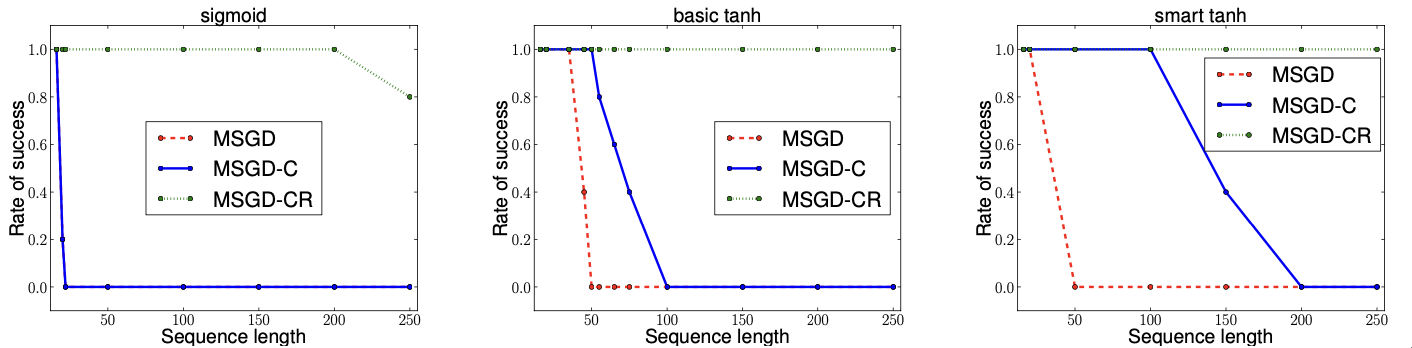
\includegraphics[width=0.9\textwidth]{figures/results.png}
  %\vspace{0.2cm}
  \captionof{\\Fig.7:Rate of success-temporal order problem vs sequence length for different initializations 
  %(left to right: sigmoid, basic tanh and smart tanh)
  }
\end{center}
 % \vspace{0.5cm}



    \end{block}

    \begin{block}{5. Relevance today \& SOTA techniques}
        %%% SUMMARY
        % \begin{table}[h!]
        % \centering
        % \begin{tabular}{|c|c|c|}
        % \hline
        % \textbf{Technique} & \textbf{Advantages} & \textbf{Disadvantages} \\ \hline
        % Gradient Clipping & Prevents exploding gradients & Requires tuning of threshold \\ \hline
        % Regularization & Mitigates vanishing gradients & May not fully prevent instability \\ \hline
        % Initialization Strategies & Improves convergence & Sensitive to parameter choice \\ \hline
        % \end{tabular}
        % \caption{Comparison of Techniques for Addressing Gradient Issues in RNNs}
        % \end{table}

 
            %%% reorganized bullet points below in more space-efficient way
        \vspace{.2em}
            \begin{tabular}{@{}ll@{}}
                \textbf{- Exploding gradients:} & \textbf{Clipping is still relevant!} \\
                \vspace{.3em}
                \textbf{- Vanishing gradients:} & 
                    \begin{minipage}[t]{0.8\textwidth} 
                        \textbf{More recent alternatives to regularization:}\\[0.3em]
                        \begin{tabular}{@{}lll@{}}
                        % $\bullet$ Residual connections & $\bullet$ Gating mechanisms   & $\bullet$ Attention mechanism \\
                        % $\bullet$ Gradient checkpointing   & $\bullet$ Layer normalization     & $\bullet$ Positional encoding \\
                        $\bullet$ Residual connections [5]     & $\bullet$ Gating mechanisms [6,7] \\
    $\bullet$ Layer normalization   [8]  & $\bullet$ Gradient checkpointing [9] \\
    $\bullet$  Attention mechanism   [10,11]   & $\bullet$ Positional encoding [10,12,13]
                        \end{tabular}
                    \end{minipage} 
                \end{tabular}
                
                \end{block}

    \begin{block}{6. References}
    % \begin{itemize} 
        % \item 
        \scriptsize{
        % \footnotesize{
        \justifying {[1]Bengio,Y., Simard,P., and Frasconi,P. (1994). Learn- ing long-term dependencies with gradient descent is difficult. IEEE Transactions on Neural Networks , 5(2), 157–166.}\\
        \justifying {[2]Hochreiter,S. and Schmidhuber,J. (1997).Long short-term memory.Neural Computation, 9(8), 1735–1780.}\\
        \justifying {[3]Boulanger-Lewandowski,N., Bengio,Y., and Vincent,P. (2012). Modeling temporal dependencies in high- dimensional sequences: Application to polyphonic music generation and transcription.In Proceed- ings of the Twenty-nine International Conference on Machine Learning (ICML’12).ACM.}\\
        \justifying {[4]Mikolov, T., Sutskever, I., Deoras, A., Le, H.-S., Kombrink, S. and Cernocky, J.(2012). Subword language modeling with neural networks.preprint (http://www.fit.vutbr.cz/imikolov/rnnlm/char.pdf).}}\\
        \justifying{[5] He, Kaiming, et al. "Deep residual learning for image recognition." %Proceedings of 
        the IEEE conference on computer vision and pattern recognition. 2016.}\\
        \justifying{[6] Cho, Kyunghyun, et al. "Learning phrase representations using RNN encoder-decoder for statistical machine translation." arXiv preprint arXiv:1406.1078 (2014).}\\
        \justifying{[7] Hochreiter, Sepp, and Jürgen Schmidhuber. "Long short-term memory." Neural computation 9.8 (1997): 1735-1780.}\\
        \justifying{[8] Ba, Jimmy Lei, Jamie Ryan Kiros, and Geoffrey E. Hinton. "Layer normalization." arXiv preprint arXiv:1607.06450 (2016).}\\
        \justifying{[9] Chen, Tianqi, et al. "Training deep nets with sublinear memory cost." arXiv preprint arXiv:1604.06174 (2016).}\\
        \justifying{[10] Vaswani, Ashish, et al. "Attention is all you need." Advances in neural information processing systems 30 (2017).}\\
        \justifying{[11] Bahdanau, Dzmitry, Kyunghyun Cho, and Yoshua Bengio. "Neural machine translation by jointly learning to align and translate." arXiv preprint arXiv:1409.0473 (2014).}\\
         \justifying{[12] Devlin, Jacob, et al. "Bert: Pre-training of deep bidirectional transformers for language understanding." Proceedings of the 2019 conference of the North American chapter of the association for computational linguistics: human language technologies, volume 1 (long and short papers). 2019.}\\
         \justifying{[13] Su, Jianlin, et al. "Roformer: Enhanced transformer with rotary position embedding." Neurocomputing 568 (2024): 127063.
}
        
    % \end{itemize}
    

    \end{block}
    
        

    %\end{block}
    \hspace{2em}
  \end{column}
  
  \end{columns}
\end{frame}

\end{document}





